%%%%%%%%%%%%%%%%%%%%%%%%%%%%%%%%%%%%%%%%%%%%%%%%%%%%%
%   RESULTADOS PARCIAIS
%%%%%%%%%%%%%%%%%%%%%%%%%%%%%%%%%%%%%%%%%%%%%%%%%%%%%

\chapter{Resultados}

Os estudos fotométricos e espectroscópicos para uma grande maioria dos objetos que compõem as Categorias do Catálogo Arp \& Madore no Universo local (z $<$ 0.1), são ainda insuficientes para tirarmos conclusões ao nível de detalhamento existente nas classes morfológicas do tipo Hubble. As peculiaridades observadas e que compõem as Categorias são diversas e carecem de dados que possam fomentar uma melhor discussão. Portanto, as conclusões obtidas nesse trabalho (ainda que parciais) e a organização das informações em um sistema Web, procuram contribuir para este propósito, sendo apresentadas nos campos da fotometria e da espectroscopia.

\section{Fotometria}

As imagens recolhidas em diversas bandas espectrais permitiu descrever um primeiro cenário fotométrico para os objetos da Categoria 7. As imagens do SDSS dispõem de informação da banda B, que possibilita uma análise dos componentes de maior energia, e da banda R, componentes mais avermelhados, portanto de natureza mais fria (as imagens desta última banda não estão presentes no mosaico construído). Já as imagens do 2MASS e Wise, fornecem informações de estrelas velhas e poeira, a depender da banda. Com o Galex evidenciamos estruturas de altas energias, como estrelas do tipo O e B ou
galáxia com núcleo ativo.

As bibliotecas ``astroquery`` do python foram usadas para o download das imagens em formato FITS, que é a extensão amplamente usada na Astronomia. A manipulação dessas imagens foi feita com o pacote "astropy.io". Analisamos imagens nas bandas J e K do 2MASS, B e R do DSS2, NUV no GALEX e 22 microm do WISE, como podem ser vistas no Apêndice A. Estas identificações preliminares foram importantes pois revelaram como um primeiro resultado que muitas galáxias, apesar da presença do jato, não apresentam evidências claras de estruturas energéticas produzidas pelas estrelas jovens O e B, ou de núcleo ativos associados a buracos negros centrais. As Figuras 7.1 e 7.2 ilustram esses resultados. Como podemos explicar fisicamente essas características? As imagens representam as seguintes bandas, da esquerda para a direita. Superior: DSS2 Blue, 2MASS-J e 2MASS-K. Inferior: WISE 3.4, Wise 2.2 e GALEX FAR UV.

\begin{figure}[H]
	\centering	
    \caption{Análise fotométrica para a galáxia AM 0233-453}
    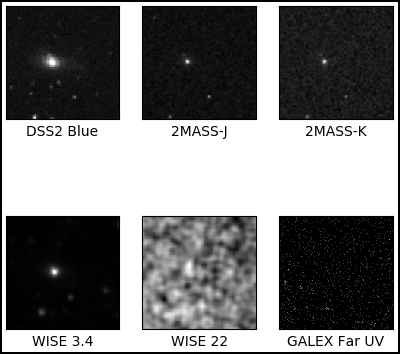
\includegraphics[width=1.0\textwidth]{figuras/am0233-453.png}
    \begin{center}
        \normalsize Fonte: Próprio Autor (2018)\\Bandas espectrais para a galáxia AM 0233-453. Note que a informação de alta energia esperada no GALEX é praticamente nula, caracterizando este objeto como uma galáxia sem atividade nuclear.
    \end{center}
	\label{fig:sbmt-moses}
\end{figure}

\begin{figure}[H]
	\centering	
    \caption{Análise fotométrica para a galáxia AM 0256-364}
    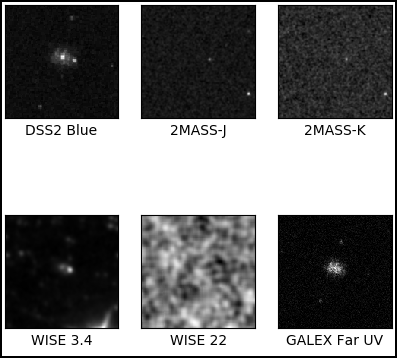
\includegraphics[width=1.0\textwidth]{figuras/am0256-354.png}
   	\begin{center}
        \normalsize Fonte: Próprio Autor (2018)\\Bandas espectrais para a galáxia AM 0256-364. Note, neste caso, que a informação de alta energia esperada no GALEX é bastante significativa, revelando que este objeto possui atividade nuclear e extranuclear.
    \end{center}
	\label{fig:sbmt-moses}
\end{figure}

\subsection{Atividade Nuclear e Jatos em Galáxias}

De uma maneira geral, podemos afirmar que praticamente todas as galáxias apresentam uma vasta coleção de estrelas na região central (incluindo também o bojo), tornando-a, dessa maneira, muito brilhante. No espectro eletromagnético, boa parte dessa dessa radiação é emitida na banda do visível, sendo uma resposta das estrelas presentes nessas regiões. Acontece, porém, que algumas galáxias apresentam o núcleo muito mais brilhante do que o esperado, não apenas no óptico, como no caso das chamadas galáxias normais,  
mas praticamente em todas bandas espectrais, dos raios gama as emissões em radio. No entanto, essa evidência observacional não pode ser explicada simplesmente pela alta concentração de estrelas na região central desses objetos. Logo, se a origem não é estelar (térmica, via lei de Planck), qual seria o mecanismo físico dessa radiação?

Tais galáxias, cujos centros emitem gigantescas quantidades de radiação e que, curiosamente, apresentam variabilidades (flutuações rápidas em intensidade), não apresentam espectros térmicos (na verdade, seguem uma lei de potência) e são denominados de galáxias ativas, e as regiões centrais de "Núcleos Ativos de Galáxias” (AGN: Active Galactic Nuclei). Estatisticamente, cerca de 10\%  das galáxias conhecidas são ativas, e são classificadas, com uma descrição muito breve, em LINERS (sendo objetos cujo mecanismo de excitação das linhas não está completamente clara, incluindo fotoionização por uma lei de potência de contínuo diluída, choques, fluxos de resfriamento e também por fotoionização por estrelas muito quentes (Wolf-Rayet) ou normais, do tipo O), Seyferts (galáxias espirais, onde o espectro nuclear apresenta linhas de emissão alargadas, indicando rápidos movimentos dos gases internos, além de um contínuo não térmico muito intenso no ultravioleta), Radiogaláxias (com emissões radio muito intensas, apresentando jatos de matéria que saem da fonte central situada no núcleo da galáxia), Quasares (de aparência estelar no óptico, possuem espectros com linhas alargadas e grandes redshifts, indicando que se encontram muito distantes) e objetos BL Lacertae (sendo também fontes de radio, com espectro não térmico contendo linhas de emissão e/ou absorção). Um recente review (incluindo também as referências) pde ser encontrada em \cite{padovani2017active}.

Uma grande fração de todas as galáxias espirais exibem um espectro nucelar com emissões de linhas se assemelham a regiões HII fotoionizadas. Estes objetos são chamados de núcleos de regiões HII, ou, para os casos excepcionalmente luminosos, núcleos Starburst. Algumas galáxias também contêm discretas regiões HII circunestelar, referidos geralmente como "hotspots". Contudo, apesar de possuírem regiões de emissão nuclear, não são caracterizados como um AGN.

No que tange a fonte de energia interna desses objetos, a comunidade astronômica aceita a ideia de que a origem da atividade nuclear está associada a presença de um buraco negro  supermassivo central, de milhões de massa solar, onde o gás acelerado cai no buraco negro e forma um disco de acreção em rotação. Amparado nas leis da Física, a medida que o gás espirala para o centro, ele transforma a energia gravitacional em energia cinética, acelerando, aquecendo e liberando enormes quantidades de  
energia. Não obstante, parte do gás que foi acretado pode ser ejetado em altas velocidades em direções perpendiculares ao disco de acreção, formando os famosos jatos e os lóbulos observados em muitas galáxias ativas. Uma possível explicação para a colimação dos jatos está associada a presença de fortes campos magnéticos originados no disco. Contudo, é importante salientar que toda energia é irradiada antes da matéria cair no horizonte de eventos do buraco negro, uma fronteira teórica ao redor deste a partir da qual a força gravitacional é tão forte que, nada, nem mesmo a luz, pode escapar pois a velocidade é inferior à velocidade de escape do buraco negro.

A acreção de matéria representa um processo extremamente eficiente em converter matéria em energia: cálculos refinados mostram que nesse processo, a energia liberada é da ordem de 0,1mc$^{2}$, quando comparada com a taxa de reação nuclear mais energética conhecida, a transformação de quatro núcleos de hidrogênio em um núcleo de hélio, que é da ordem de 0,007mc$^{2}$. Portanto, quando o buraco negro consumir toda matéria circundante, a atividade nuclear automaticamente cessa, restando apenas um buraco negro quiescente em seu centro. Este é o mesmo processo básico, proposto Salpeter e  Zel'dovich: (1964).

Apesar dessa descrição responder muito bem a presença dos jatos em galáxias com núcleos ativos, como ainda explicar a presença do jato ópticos em galaxias normais, como muito daquelas encontradas na Categoria 7?

Diversos modelos teóricos foram propostos nas últimas décadas para explicar a presença dos jatos, com evidências para a rotação rápida dos buracos negros supermassivos. Um consenso geral esta sendo formado de que os jatos são fundamentalmente fenômenos cuja origem está relacionada aos processos eletromagnéticos no disco de acreção ao redor do buraco negro central, e não apenas como uma consequência de processos puramente hidrodinâmicos. 

Como não pretendemos construir um novo modelo que possa envolver tais quantidades físicas, esperamos contribuir com informações fotométricas e espectroscópicas que possam fomentar novas discussões sobre as peculiaridades observadas nos objetos da Categoria 7.

\subsection{Diagrama de Cores}

Um mapa do tipo cor-cor é importante pois permite obter algumas informações independentes da distância do objeto estudado. O que estamos denominando de cor neste trabalho, consiste na diferença entre o brilho do objeto em bandas
diferentes do especto eletromagnético. Assim, podemos analisar as propriedades dos objetos selecionados e averiguar se existe alguma segregação nestes. 

Ao separar em dois conjuntos a nossa amostra fotométrica (objetos com atividade nuclear e sem atividade nuclear), não apenas com a ajuda das imagens, mas também com a espectroscopia, geramos, automaticamente, uma segregação. Embora a morfologia peculiar não esteja presente no diagrama presente na Figura \ref{fig:cores} (o que pode ser pensado como algo similar para todas as Categorias do Catálogo Arp \& Madore), é possível, pelo menos, verificar que esta segregação desaparece e percebemos que os objetos permeiam entre os diversos níveis de energia nuclear, revelando que os mesmos, apesar de sua característica peculiar, comunga de propriedades semelhantes as diversas outras classes morfológicas de Hubble. É importante frisar que não estamos comparando classes morfológicas, mas sim uma ideia referente as atividades (ou não) presentes no núcleo. Percebe-se também que o autor do diagrama \cite{wright2010wide}, não fez qualquer separação entre subclassificações existentes nas elípticas ou nas espirais.

\begin{figure}[H]
	\centering	
    \caption{Diagrama cor-cor, mostrando a localização da classificação de diferentes tipos morfológicos. Nesta, incluímos as galáxias peculiares desse estudo.}
    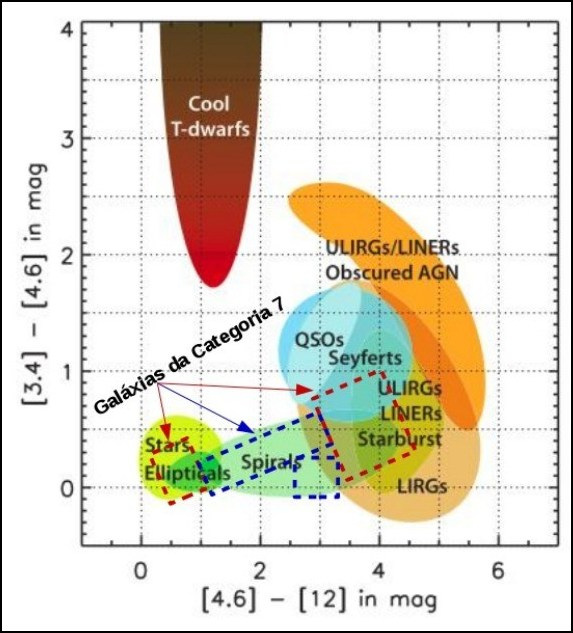
\includegraphics[width=1.0\textwidth]{figuras/coresm.jpg}
   	\begin{center}
        \normalsize Fonte: \cite{wright2010wide} (modificado).\\A cor W1-W2 ([3.4]-[4.6] in mag), fornece informação sobre o conteúdo mais azulado, enquanto a cor W2-W3 ([4.6]-[12] in mag) fornece indícios de conteúdos mais avermelhado. Portanto, podemos inferir sobre a população estelar das galáxias estudadas, representadas pelas regiões tracejadas sobre a Figura.
    \end{center}
	\label{fig:cores}
\end{figure}

O diagrama cor-cor na banda do WISE (Figura 7.3), fornece uma separação clara entre os principais tipos morfonológicos/espectrais conhecidos. Apesar de tratar tipos morfológicos, também fornecem informações sobre o tipo de atividade nuclear (se presente ou não) nestas classes. Portanto, o lado esquerdo do gráfico exprimi atributos de galáxias velhas, sem atividade nuclear e extranuclear. Já no extremo oposto, temos o perfil
de galáxias com forte atividade nuclear ou extranuclear. Fica claro que os objetos estudados não apenas permeiam por estes dois grupos, mas também possuem características semelhantes (em cores) com vários tipos morfológicos. O próximo passo consiste em conhecer o conteúdo das populações estelares presentes nesses objetos através do código de síntese espectral STARLIGHT.

\section{Síntese Espectral}

O código STARLIGHT cria e ajusta ao espectro observado e devidamente calibrado, um espectro sintético que representa uma combinação linear de SSPs extraídas de uma grade de modelos semi-empíricos. O resultado esperado da síntese espectral fornece um vetor de população ($\vec{x}$), que representa a fração de contribuição das SSPs utilizadas no ajuste de diferentes idades (muito jovens, jovens, intermediárias e velhas), e o próprio espectro sintético (M$_{\lambda}$). Outros resultados estão relacionados com a velocidade de dispersão da galáxia e o vetor de massa ($\vec{\mu}$), que representa a fração de massa de cada SSP tomada no ajuste.

Para calcularmos os espectros sintéticos de nossa amostra (observada e da literatura), o código ajusta a melhor combinação de SSPs para fazer o melhor ajuste possível ao espectro de entrada, fornecendo várias propriedades 
físicas de interesse, como a massa estelar atual, a extinção estelar, as distribuições e médias das idades (t) e metalicidades (Z) das SSPs, i.e., as frações de massa e de luminosidade para cada SSP de certa idade e metalicidade. Desse modo, podemos construir uma possível história de formação estelar do sistema físico estudado, bem como inferir sobre a evolução temporal do enriquecimento químico traçado pelas populações estelares do sistema (relação entre Z e t).

Como os objetos da literatura são estudos baseados em grandes surveys, já reduzidos e calibrados, selecionamos um conjunto de observações realizadas no OPD-LNA/MCTIC para servir de controle, no que tange a redução e a síntese espectral. O desejável seria que todo o conjunto de objetos do OPD/LNA-MCTIC estivesse presente na amostra do 6dFGS, o que não foi possível. Apenas cinco objetos possuem espectros no referido survey. Contudo, as informações são igualmente importantes para compilar uma primeira base de dados espectroscópicos para essa Categoria.

As Figuras \ref{fig:normal} e \ref{fig:ativas} ilustram dois exemplos das sínteses espectrais conduzidas para dois objetos em comum da amostragem, AM 2359-381 (galáxia normal) e AM 0633-352 (galáxia ativa). Os detalhes das sínteses são dadas nas próprias Figuras.

\begin{figure}[H]
	\centering	
    \caption{Síntese espectral da galáxia peculiar AM 2359-381.}
    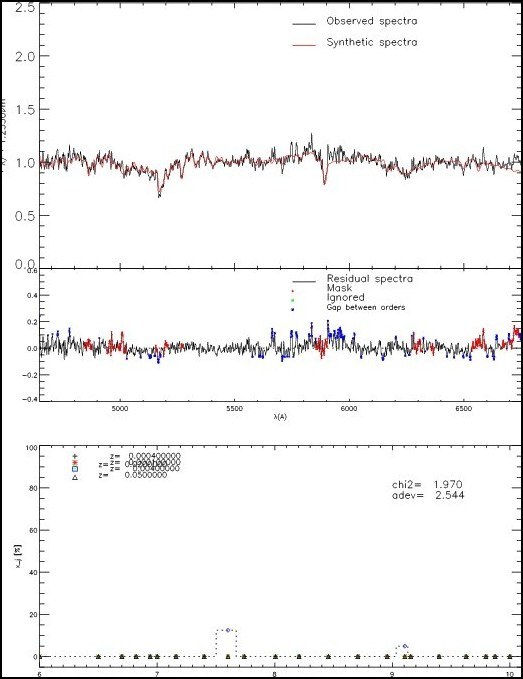
\includegraphics[width=0.85\textwidth]{figuras/normal.jpg}
   	\begin{center}
        \normalsize Fonte: Próprio Autor. painel Superior.\vskip 0.5cm Painel Superior: A linha preta sólida representa o espectro observado e, em vermelho, o modelado (sintético). Painel Central: As linhas vermelhas representam as máscaras usadas em regiões de linhas de emissão, extrações ruins oriundas das reduções, linhas telúricas, etc.; as linhas verdes significam regiões que foram ignoradas durante a síntese, previamente definidas pelo usuário, e as azuis, os possíveis "gap" entre as ordens durante o processo de ajuste espectral. Painel Inferior: As diferentes metalicidades encontradas em função do vetor de população (eixo y) e do logaritmo da idade (em anos).
    \end{center}
	\label{fig:normal}
\end{figure}


\begin{figure}[H]
\centering	
\caption{Síntese espectral da galáxia peculiar AM 0633-352}
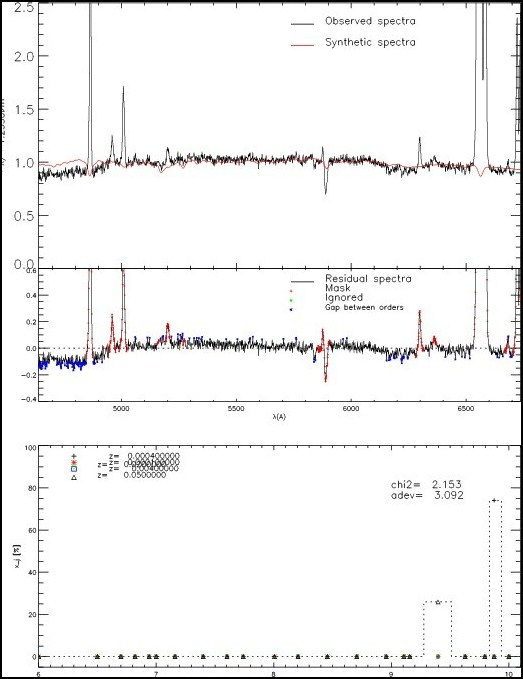
\includegraphics[width=0.85\textwidth]{figuras/ativas.jpg}
\begin{center}
   \normalsize Fonte: Próprio autor. Ver comentários na Figura 7.4
    \end{center}
\label{fig:ativas}
\end{figure}

A Figura \ref{fig:vetorpop} ilustra a distribuição das idades (por Grupo) a partir da síntese espectral, o que permite inferir diretamente sobre a população estelar com maior predominância na Categoria 7. Podemos perceber que uma fração considerável dos objetos já consumiram as reservas de gás, apresentando assim, estrelas velhas e material interestelar frio, tal como as galáxias
elípticas. Ressaltamos que uma parcela dos objetos estão superpostos nesta região na Figura 7.3. Por outro lado, um outro grupo de galáxias apresentam elementos que favorecem à formação de estrelas, similares a que observamos
nos braços de galáxias espirais e nas morfologias mais a direita no diagrama. 


\begin{figure}[H]
	\centering	
    \caption{Vetor de População da Amostra.}
    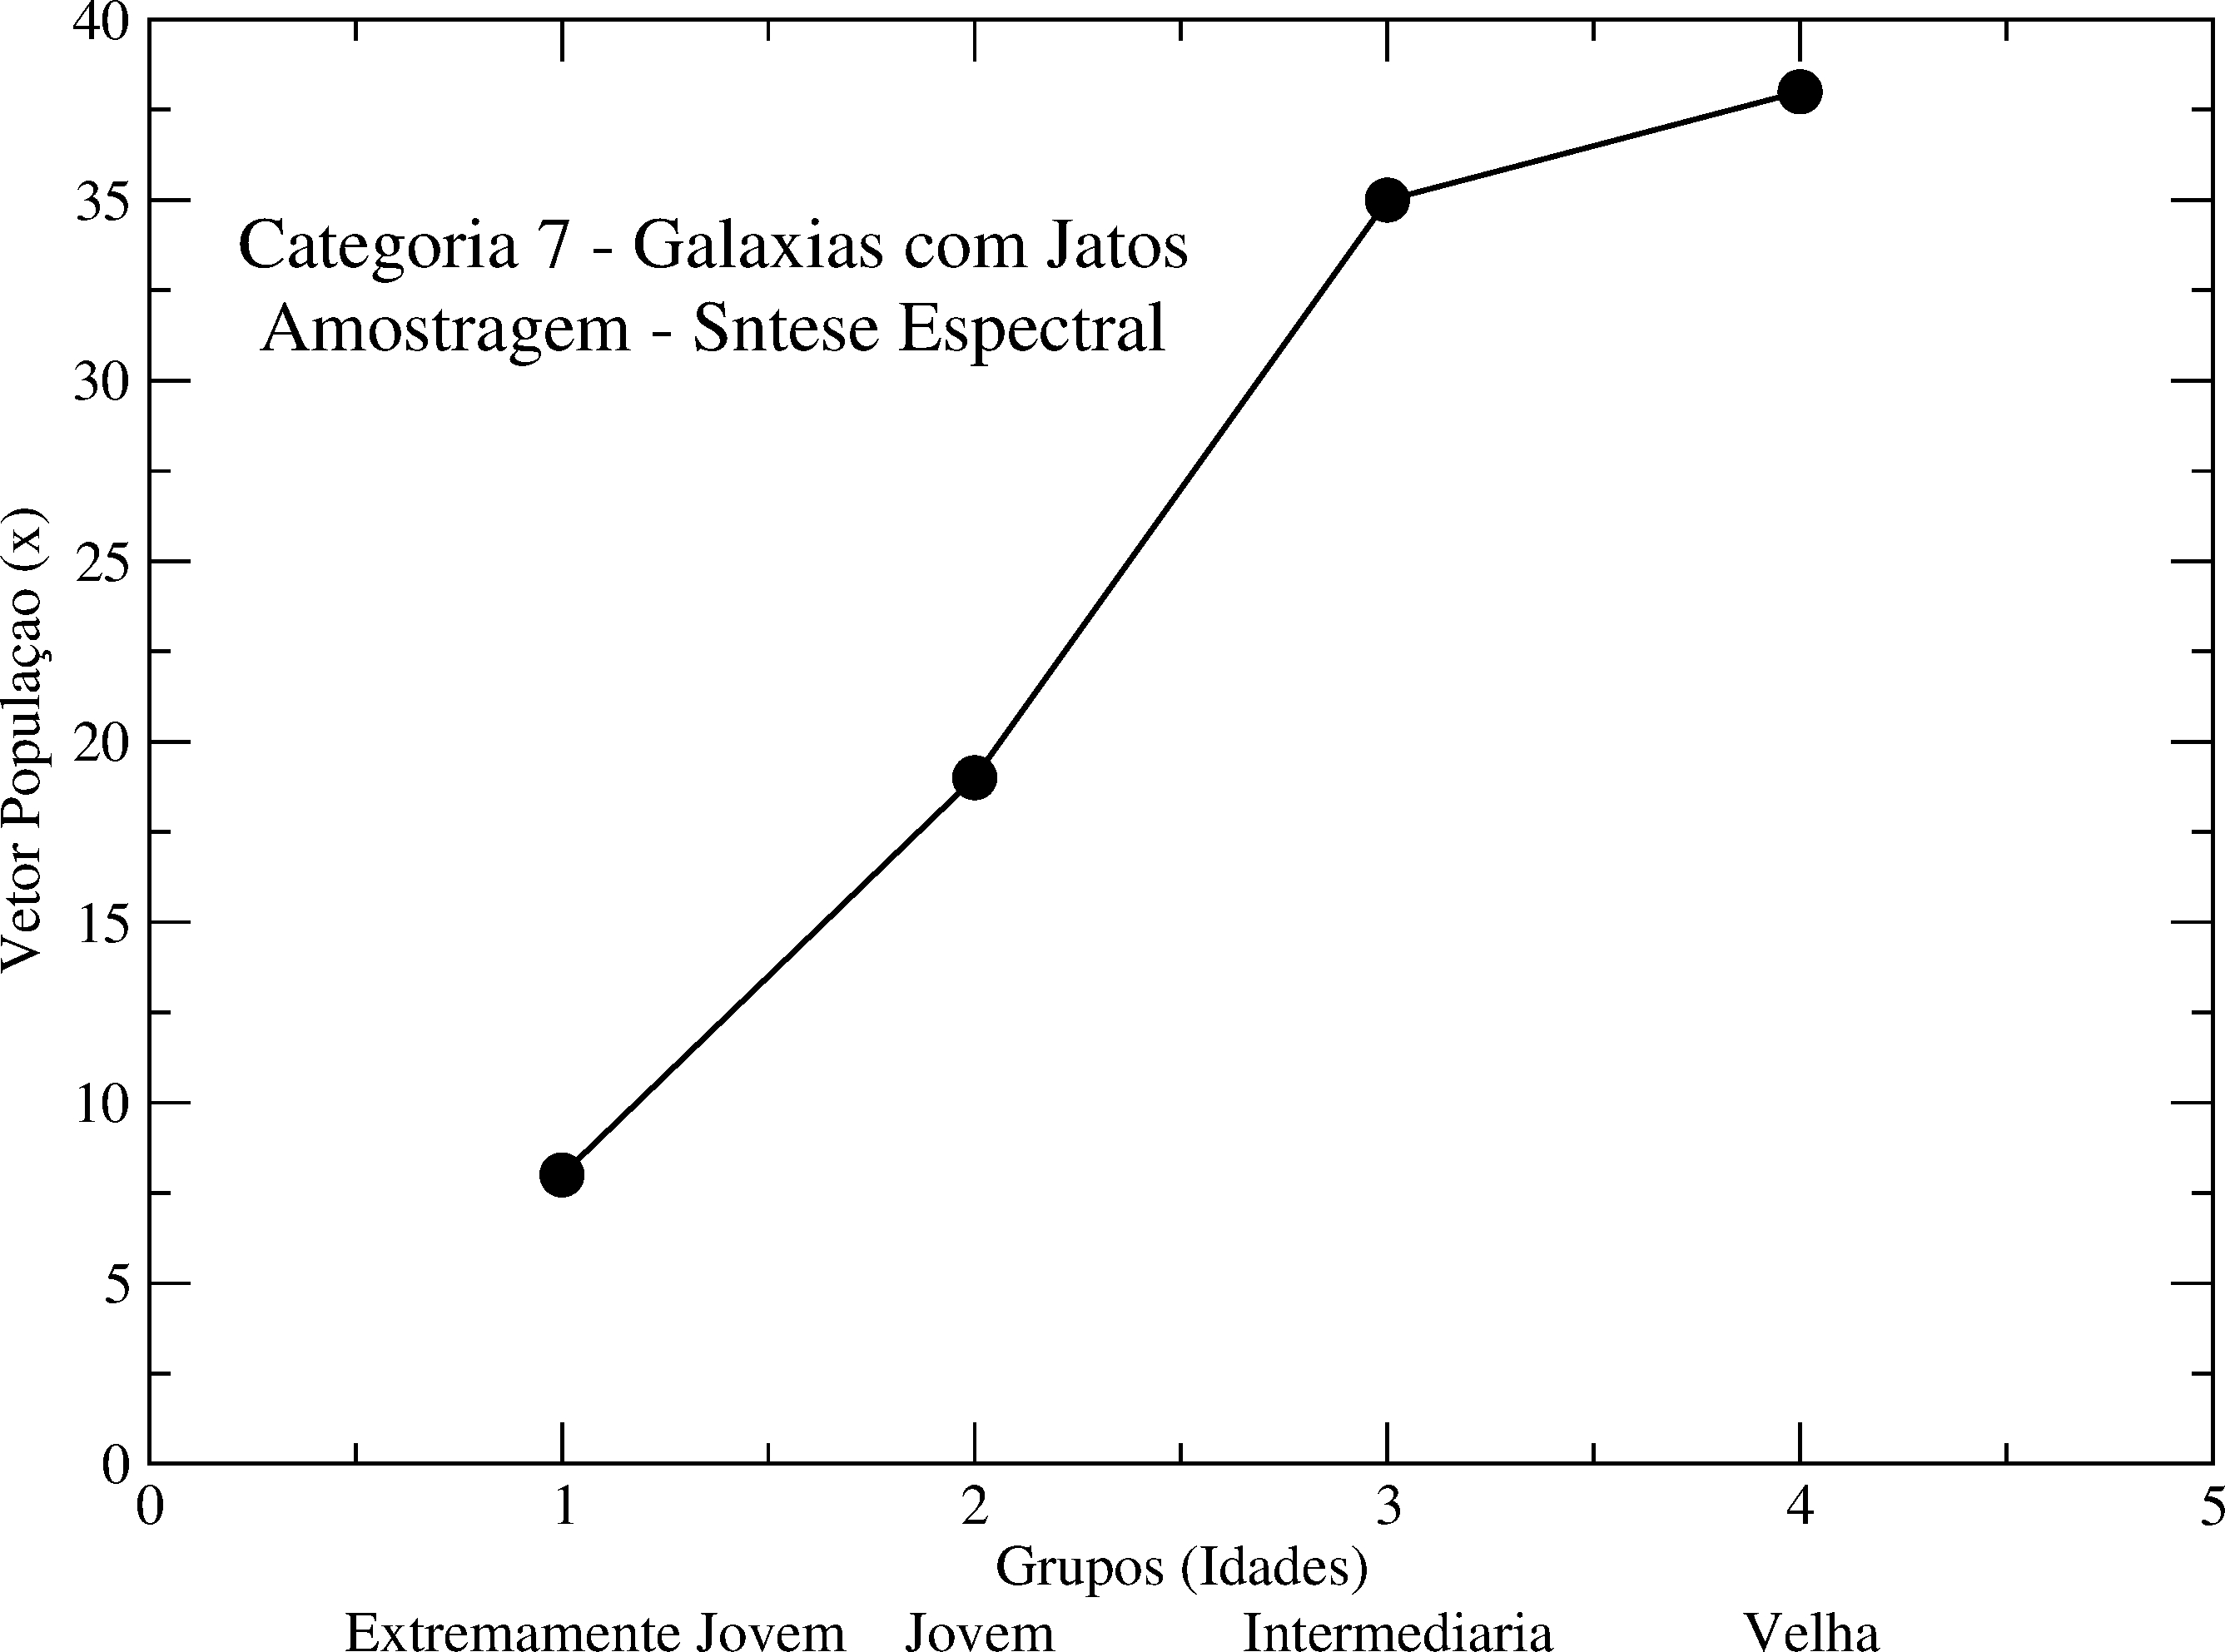
\includegraphics[width=0.8\textwidth]{figuras/vetorpop.jpg}
    \vskip 0.5cm
   	\begin{center}
        \normalsize Fonte: Autor (própria). Predominância das populações na amostra selecionada da Categoria 7. Os Grupos de Idade seguem os seguintes intervalos: G1 - Extremamente Jovens, x$_M${$_j$} 
(t \le 1 $\times$10$^8$ anos); G2 - Jovens, x{$_J$} (1$\times$10{$^8$} < t \le 5$\times$10{$^8$} anos); G3 - Idades Intermediárias, x{$_I$}, (5$\times$10$^8$ < t \le 2$\times$10{$^9$} anos) e G4 - Velhas, x{$_O$} (t > 2$\times$10$^9$ anos).
    \end{center}
	\label{fig:vetorpop}
\end{figure}

\section{Algumas Questões sobre os Jatos nas Galáxias Estudadas.} 

Que tipo de jato, envolvendo uma categoria particular de galáxias classificadas como peculiares, estamos discutindo neste trabalho? Será que as peculiaridades observadas no óptico são diferentes, no que tange aos mecanismos de produção, dos jatos relativı́sticos extragaláticos observados em radiogaláxias?

Um jato astrofísico pode ser definido, de forma simplificada, como um escoamento de material proveniente da região central de uma galáxia. Sendo estes escoamentos colimados de plasma ejetados a velocidades relativı́sticas, emergindo dos núcleos ativos de galáxias em direções opostas, transportando enormes quantidades de massa, momentum e energia, temos, claramente os chamados jatos relativı́sticos com evidência teóricas e observacionais associadas a rotação rápida dos buracos negros supermassivos. Os processos físicos envolvidos nesses casos não são triviais e tem desafiado ao longo do tempo a nossa compreensão quanto a origem, colimação, propagação, radiação etc., além de outros processos fı́sicos envolvidos \cite{begelman1984theory, ferrari1998modeling, blandford1990physical, krolik1999active, meier2001magnetohydrodynamic, collin2006quasars} dentre outros. %(e.g.,Begelman et al., 1984, Ferrari, 1998, Blandford, 1990, Krolik, 1999, Meier et al., 2001, Collin, 2006, dentre outros).

A combinação envolvendo estudos teóricos \cite{blandford1977electromagnetic,blandford1982hydromagnetic,  begelman1984theory,  punsly1990ergosphere, ferrari1998modeling, meier2001magnetohydrodynamic} associado ao uso de complexas simulações numéricas magnetohidrodinâmicas (MHD) relativísticas \cite{koide2000general, koide2003magnetic, mckinney2004measurement, de2005magnetically, komissarov2005observations, hawley2006magnetically, mckinney2006general, mckinney2007disc, punsly2007three, tchekhovskoy2008simulations} estão fornecendo importantes pistas para a compreensão física das energias transportadas pelos jatos extragaláticos. No entanto, esta é uma tarefa árdua e toda contribuição nos campos da fotometria, espectroscopia e polarimetria são de suma importância nesse processo.

Os seguinte pontos traduzem algumas questões primárias sobre a presença dos jatos observados nessas galáxias peculiares.

\begin{enumerate}
    
    \item No caso particular das galáxias peculiares, a origem comumente associada para as morfologias esperadas encontra-se ancorada em um dos processos de interação gravitacional: colisão, fusão ou efeito de maré. Portanto, é esperado que algum desses processos perturbativos possa disparar algum mecanismo interno que culmine no jato observado. Infelizmente, nem as imagens e nem os espectros dos bancos de dados, contêm informações sobre os jatos observados. Que tipo de correlação com o espectro nuclear observado, após a síntese de população estelar, poderíamos esperar?
    
    \item Qual a origem dos jatos em galáxias peculiares normais, reveladas pelas imagens ou pela síntese espectral?
    
    \item A existência de contrapartidas em radio desses objetos poderiam levá-los a uma discussão similar já estabelecida para as radiogaláxias?

    \item Os jatos relativísticos já estudados na literatura podem permanecer altamente colimados até distâncias da ordem de centenas de kiloparsecs em relação ao centro das radiogaláxias? No caso das galáxias peculiares com jatos, as distâncias são de apenas alguns kiloparsecs. Qual a justificativa que podemos apontar para esta diferença? Será que o escoamento acretivo que deposita massa no buraco negro central, atravessado por linhas de campo magnético de grande escala, é relativamente menor?

    \item Os jatos podem exercer algum impacto no meio interestelar das galáxias hospedeiras?

\end{enumerate}

